\documentclass{beamer}
\usetheme{Madrid}

\usepackage{amsmath,amssymb,amsfonts,amsthm}
\usepackage{graphicx}
\usepackage{listings}
\usepackage{gensymb}
\usepackage[utf8]{inputenc}
\usepackage{hyperref}
\usepackage{gvv}

\begin{document}

\title{9.5.6}
\author{EE24BTECH11018 - Durgi Swaraj Sharma}
\date{}
\frame{\titlepage}

\begin{frame}
\frametitle{Question}
Find the area of the region lying above the $X$ axis and included between the circle $x^2+y^2=8x$ and inside of the parabola $y^2=4x$. \hfill \brak{12, 2018}
\end{frame}

\begin{frame}
\frametitle{Variables Used}
\begin{table}[h!] 
  \centering
  \begin{center}
    \begin{tabular}{|c|c|c|} 
        \hline
            \textbf{Point} & \textbf{Description} & \textbf{Coordinates} \\ 
        \hline
            $A$   & One end of the line segment & $A =$ \myvec{-2 \\ 0} \\ 
        \hline
            $B$   & Other end of line segment & $B =$ \myvec{0 \\ 8}\\ 
        \hline
	    $P$   & Point trisecting the line segment and closer to point \textbf{A} & $P  =$ \myvec{x_1 \\ y_1}\\ 
        \hline
	    $Q$   & The other point trisecting the line segment & $Q  =$ \myvec{x_2 \\ y_2}\\ 
	    \hline
    \end{tabular}
\end{center}  

  %\caption{Variables Used}
  \label{tab9-5.6-1}
\end{table}
\end{frame}
\begin{frame}
\frametitle{Equations}
Equation of a circle is of form $\vec{x}^{\top}\vec{V}\vec{x}+2\vec{u}^{\top}\vec{x}+f=0$ with
\begin{align}
	\vec{u}=\myvec{-4\\0}\\
	f=\norm{\vec{u}}^2-r^2\\
	\vec{V}=\myvec{1&0\\0&1}
\end{align}
\end{frame}

\begin{frame}
	\frametitle{Equations}
Equation of parabola with directrix $\vec{n}^{\top}\vec{x}=c$ is given by,
\begin{align}
	g\brak{\vec{x}}=\vec{x}^{\top}\vec{V}\vec{x}+2\vec{u}^{\top}\vec{x}+f=0\\
	\vec{V}=\norm{\vec{n}}^2\vec{I}-e^2\vec{n}\vec{n}^{\top}\\
	\vec{u}=ce^2\vec{n}-\norm{\vec{n}}^2\vec{F}\\
	f=\norm{\vec{n}}^2\norm{\vec{F}}^2-c^2e^2
\end{align}
and for the parabola $y^2=4x$, equation of directrix is, $\myvec{-1&0}\vec{x}=1$
\begin{align}
	\vec{V}&=\myvec{0&0\\0&1}\\
	\vec{u}&=\myvec{-2\\0}\\
	f&=0
\end{align}
\end{frame}

\begin{frame}
	\frametitle{Solving}
The intersection of two conics with parameters $\vec{V}_i,\vec{u}_i,f_i, i=1,2$ is defined as,
\begin{align}
	\vec{x}^{\top}\brak{\vec{V}_1-\vec{V}_2}\vec{x}+2\brak{\vec{u}_1-\vec{u_2}}^{\top}\vec{x}+\brak{f_1-f_2}=0
\end{align} 
On solving we get the points of intersection to be $\myvec{0\\0},\myvec{4\\4}.$
\begin{figure}[h!]
   \centering
   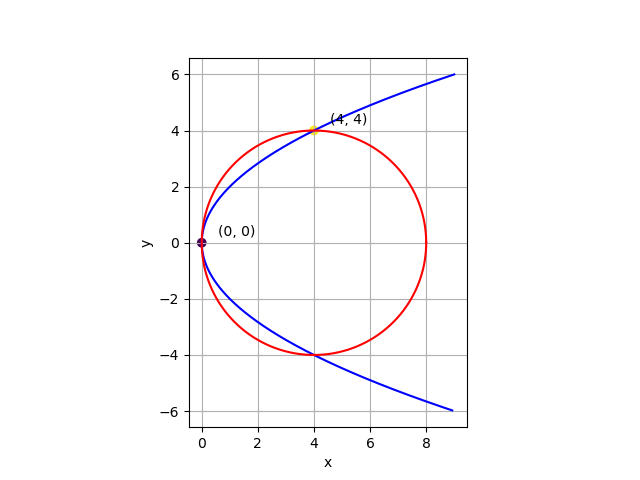
\includegraphics[width = 0.5\linewidth]{figs/fig1.png}
	%\caption{Found points}
   \label{stemplot}
\end{figure}
\end{frame}

\begin{frame}
	\frametitle{Solving}
Area between the two curves above $X$ axis is,
\begin{align}
	&\int_0^4 2\sqrt{x} dx- \int_0^4 \sqrt{x^2-8x} dx = \frac{12\pi-32}{3} \approx 1.899.
\end{align}
The area between the curves $y^2=4x, x^2+y^2=8x$ above the $X$ axis is around 1.899 units.
\end{frame}
\begin{frame}
	\frametitle{Graph}
\begin{figure}[h!]
   \centering
   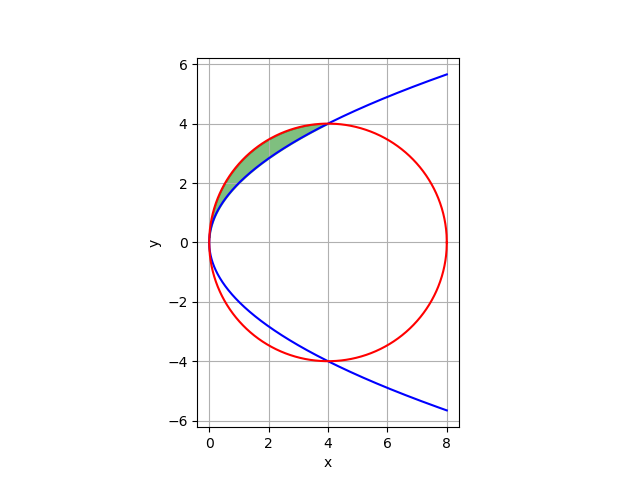
\includegraphics[width = 0.7\linewidth]{figs/fig.png}
   \caption{Required area}
   \label{stemplot}
\end{figure}
\end{frame}

\definecolor{codegreen}{rgb}{0,0.6,0}
\definecolor{codegray}{rgb}{0.5,0.5,0.5}
\definecolor{codepurple}{rgb}{0.58,0,0.82}
\definecolor{backcolour}{rgb}{0.95,0.95,0.92}


\lstset{
    language=C,
    basicstyle=\footnotesize\ttfamily,
    backgroundcolor=\color{backcolour},
    commentstyle=\color{codegreen},
    keywordstyle=\color{blue},
    numberstyle=\tiny\color{codegray},
    stringstyle=\color{codepurple},
    breakatwhitespace=false,
    breaklines=true,
    captionpos=b,
    keepspaces=true,
    numbers=left,
    numbersep=5pt,
    showspaces=false,
    showstringspaces=false,
    showtabs=false,
    tabsize=2
}
\begin{frame}[fragile,allowframebreaks]
\frametitle{C Code}
\lstinputlisting[label=mycode1]{codes/generate.c}
\end{frame}

\definecolor{codegreen}{rgb}{0,0.6,0}
\definecolor{codegray}{rgb}{0.5,0.5,0.5}
\definecolor{codepurple}{rgb}{0.58,0,0.82}
\definecolor{backcolour}{rgb}{0.95,0.95,0.92}

\lstset{
    language=Python,
    basicstyle=\ttfamily\small,
    keywordstyle=\color{blue},
    stringstyle=\color{codepurple},
    commentstyle=\color{codegreen},
    backgroundcolor=\color{backcolour},
    breaklines=true,
    breakatwhitespace=true,
    tabsize=4
}

\begin{frame}[fragile,allowframebreaks]
\frametitle{Python Code}
\lstinputlisting[label=mycode1]{codes/plot.py}
\end{frame}

\end{document}
